\documentclass{standalone}
\usepackage{tikz}
\usetikzlibrary{patterns, positioning}
\usepackage[sfdefault]{ClearSans} %% option 'sfdefault' activates Clear Sans as the default text font
\usepackage[T1]{fontenc}

\begin{document}
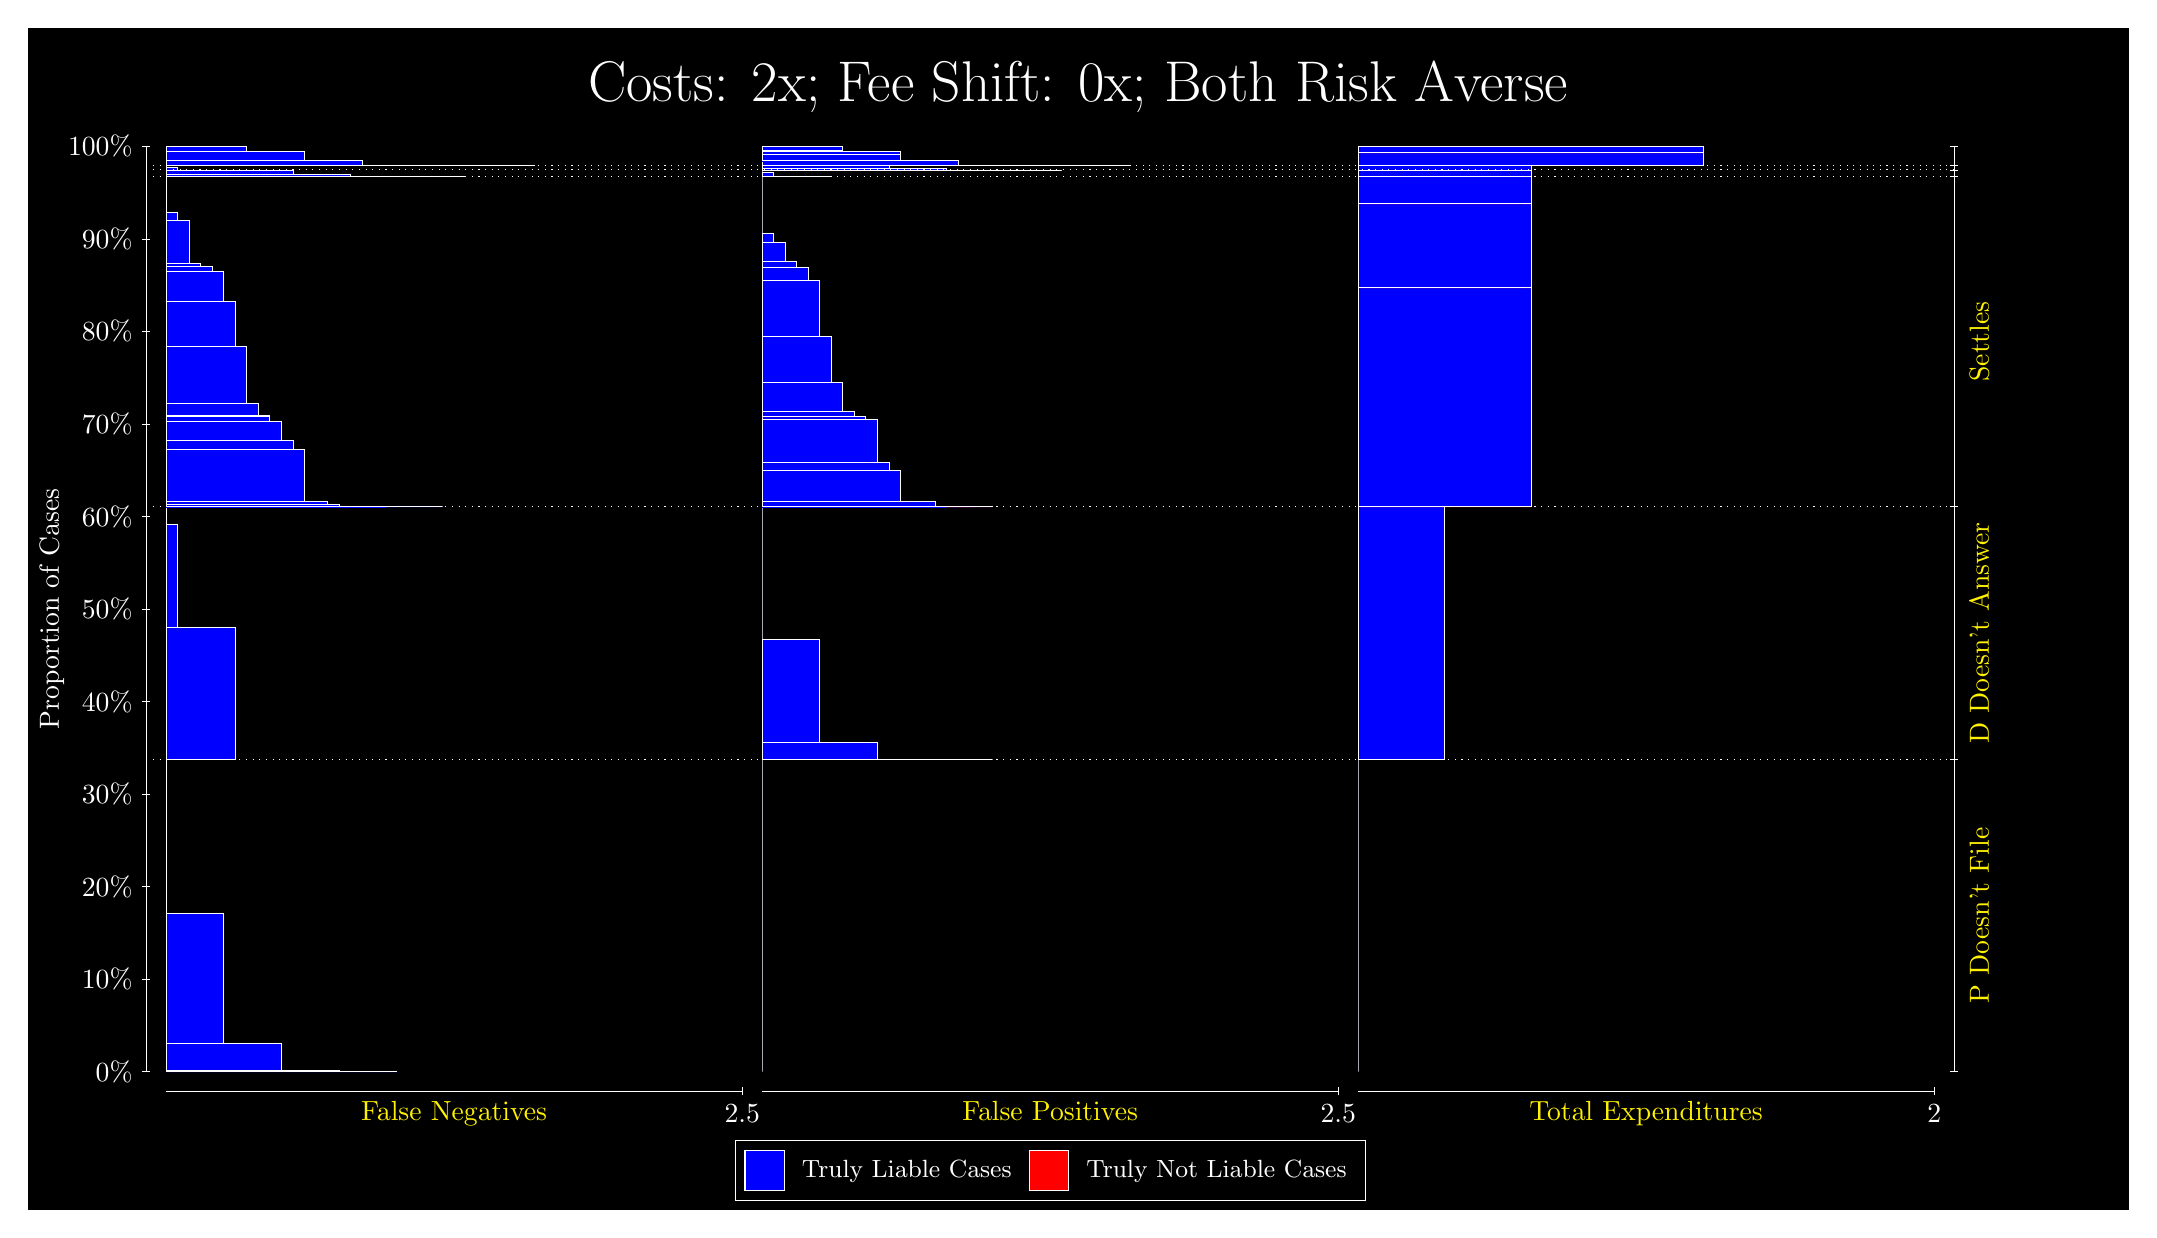
\begin{tikzpicture}
\draw[fill=black] (0,0) rectangle (26.667,15);
\draw[text=white] (0,13.5) rectangle (26.667,15) node[midway] {\huge Costs: 2x; Fee Shift: 0x; Both Risk Averse};
\draw[white, very thin] (1.5,1.75) -- (1.5,13.5);
\node[rotate=90, text=white, anchor=center] at (0.3, 7.625) {Proportion of Cases};
\draw[white, very thin] (1.45,1.75) -- (1.55,1.75);
\node[text=white, anchor=east] at (1.45, 1.75) {0\%};
\draw[white, very thin] (1.45,2.925) -- (1.55,2.925);
\node[text=white, anchor=east] at (1.45, 2.925) {10\%};
\draw[white, very thin] (1.45,4.1) -- (1.55,4.1);
\node[text=white, anchor=east] at (1.45, 4.1) {20\%};
\draw[white, very thin] (1.45,5.275) -- (1.55,5.275);
\node[text=white, anchor=east] at (1.45, 5.275) {30\%};
\draw[white, very thin] (1.45,6.45) -- (1.55,6.45);
\node[text=white, anchor=east] at (1.45, 6.45) {40\%};
\draw[white, very thin] (1.45,7.625) -- (1.55,7.625);
\node[text=white, anchor=east] at (1.45, 7.625) {50\%};
\draw[white, very thin] (1.45,8.8) -- (1.55,8.8);
\node[text=white, anchor=east] at (1.45, 8.8) {60\%};
\draw[white, very thin] (1.45,9.975) -- (1.55,9.975);
\node[text=white, anchor=east] at (1.45, 9.975) {70\%};
\draw[white, very thin] (1.45,11.15) -- (1.55,11.15);
\node[text=white, anchor=east] at (1.45, 11.15) {80\%};
\draw[white, very thin] (1.45,12.325) -- (1.55,12.325);
\node[text=white, anchor=east] at (1.45, 12.325) {90\%};
\draw[white, very thin] (1.45,13.5) -- (1.55,13.5);
\node[text=white, anchor=east] at (1.45, 13.5) {100\%};

\draw[white, very thin] (24.457,1.75) -- (24.457,13.5);
\draw[white, very thin] (24.407,1.75) -- (24.507,1.75);
\node[anchor=west] at (24.407, 1.75) {};
\draw[white, very thin] (24.407,5.7137) -- (24.507,5.7137);
\node[anchor=west] at (24.407, 5.7137) {};
\draw[white, very thin] (24.407,8.9233) -- (24.507,8.9233);
\node[anchor=west] at (24.407, 8.9233) {};
\draw[white, very thin] (24.407,13.118) -- (24.507,13.118);
\node[anchor=west] at (24.407, 13.118) {};
\draw[white, very thin] (24.407,13.2) -- (24.507,13.2);
\node[anchor=west] at (24.407, 13.2) {};
\draw[white, very thin] (24.407,13.257) -- (24.507,13.257);
\node[anchor=west] at (24.407, 13.257) {};
\draw[white, very thin] (24.407,13.5) -- (24.507,13.5);
\node[anchor=west] at (24.407, 13.5) {};

\draw[white, very thin, fill=blue] (1.75,1.75) rectangle (4.6775,1.7501);
\draw[white, very thin, fill=blue] (1.75,1.7501) rectangle (3.9457,1.7603);
\draw[white, very thin, fill=blue] (1.75,1.7603) rectangle (3.2138,2.1036);
\draw[white, very thin, fill=blue] (1.75,2.1036) rectangle (2.4819,3.7584);
\draw[white, very thin, fill=red] (1.75,3.7584) rectangle (1.75,3.7584);
\draw[white, very thin, fill=blue] (1.75,3.7584) rectangle (1.75,5.7137);
\draw[white, very thin, fill=blue] (1.75,5.7137) rectangle (2.6283,7.3936);
\draw[white, very thin, fill=blue] (1.75,7.3936) rectangle (1.8964,8.7057);
\draw[white, very thin, fill=red] (1.75,8.7057) rectangle (1.75,8.7057);
\draw[white, very thin, fill=blue] (1.75,8.7057) rectangle (1.75,8.9233);
\draw[white, very thin, fill=blue] (1.75,8.9233) rectangle (5.2631,8.9233);
\draw[white, very thin, fill=blue] (1.75,8.9233) rectangle (4.6775,8.9234);
\draw[white, very thin, fill=blue] (1.75,8.9234) rectangle (4.5312,8.9243);
\draw[white, very thin, fill=blue] (1.75,8.9243) rectangle (4.3848,8.9243);
\draw[white, very thin, fill=blue] (1.75,8.9243) rectangle (4.092,8.9246);
\draw[white, very thin, fill=blue] (1.75,8.9246) rectangle (3.9457,8.953);
\draw[white, very thin, fill=blue] (1.75,8.953) rectangle (3.7993,8.9872);
\draw[white, very thin, fill=blue] (1.75,8.9872) rectangle (3.6529,8.9945);
\draw[white, very thin, fill=blue] (1.75,8.9945) rectangle (3.5065,9.6496);
\draw[white, very thin, fill=blue] (1.75,9.6496) rectangle (3.3602,9.7613);
\draw[white, very thin, fill=blue] (1.75,9.7613) rectangle (3.2138,10.006);
\draw[white, very thin, fill=blue] (1.75,10.006) rectangle (3.0674,10.072);
\draw[white, very thin, fill=blue] (1.75,10.072) rectangle (3.0674,10.079);
\draw[white, very thin, fill=blue] (1.75,10.079) rectangle (2.921,10.237);
\draw[white, very thin, fill=blue] (1.75,10.237) rectangle (2.7746,10.956);
\draw[white, very thin, fill=blue] (1.75,10.956) rectangle (2.6283,11.537);
\draw[white, very thin, fill=blue] (1.75,11.537) rectangle (2.4819,11.907);
\draw[white, very thin, fill=blue] (1.75,11.907) rectangle (2.3355,11.976);
\draw[white, very thin, fill=blue] (1.75,11.976) rectangle (2.3355,11.976);
\draw[white, very thin, fill=blue] (1.75,11.976) rectangle (2.1891,12.009);
\draw[white, very thin, fill=blue] (1.75,12.009) rectangle (2.0428,12.56);
\draw[white, very thin, fill=blue] (1.75,12.56) rectangle (1.8964,12.658);
\draw[white, very thin, fill=red] (1.75,12.658) rectangle (1.75,12.658);
\draw[white, very thin, fill=blue] (1.75,12.658) rectangle (1.75,13.118);
\draw[white, very thin, fill=blue] (1.75,13.118) rectangle (5.5558,13.118);
\draw[white, very thin, fill=blue] (1.75,13.118) rectangle (4.8239,13.118);
\draw[white, very thin, fill=blue] (1.75,13.118) rectangle (4.092,13.149);
\draw[white, very thin, fill=blue] (1.75,13.149) rectangle (3.3602,13.199);
\draw[white, very thin, fill=blue] (1.75,13.199) rectangle (2.6283,13.2);
\draw[white, very thin, fill=red] (1.75,13.2) rectangle (1.75,13.2);
\draw[white, very thin, fill=blue] (1.75,13.2) rectangle (2.6283,13.201);
\draw[white, very thin, fill=blue] (1.75,13.201) rectangle (1.8964,13.236);
\draw[white, very thin, fill=red] (1.75,13.236) rectangle (1.75,13.236);
\draw[white, very thin, fill=blue] (1.75,13.236) rectangle (1.75,13.257);
\draw[white, very thin, fill=blue] (1.75,13.257) rectangle (6.4341,13.257);
\draw[white, very thin, fill=blue] (1.75,13.257) rectangle (5.7022,13.257);
\draw[white, very thin, fill=blue] (1.75,13.257) rectangle (4.9703,13.261);
\draw[white, very thin, fill=blue] (1.75,13.261) rectangle (4.2384,13.317);
\draw[white, very thin, fill=blue] (1.75,13.317) rectangle (3.5065,13.44);
\draw[white, very thin, fill=blue] (1.75,13.44) rectangle (2.7746,13.496);
\draw[white, very thin, fill=blue] (1.75,13.496) rectangle (2.0428,13.5);
\draw[white, very thin, fill=red] (1.75,13.5) rectangle (1.75,13.5);
\draw[white, very thin, fill=blue] (1.75,13.5) rectangle (1.75,13.5);
\draw[white, very thin, fill=red] (9.3189,1.75) rectangle (9.3189,1.75);
\draw[white, very thin, fill=blue] (9.3189,1.75) rectangle (9.3189,5.7137);
\draw[white, very thin, fill=red] (9.3189,5.7137) rectangle (12.246,5.7137);
\draw[white, very thin, fill=blue] (9.3189,5.7137) rectangle (12.246,5.7137);
\draw[white, very thin, fill=blue] (9.3189,5.7137) rectangle (11.515,5.7147);
\draw[white, very thin, fill=blue] (9.3189,5.7147) rectangle (10.783,5.9312);
\draw[white, very thin, fill=blue] (9.3189,5.9312) rectangle (10.051,7.2434);
\draw[white, very thin, fill=blue] (9.3189,7.2434) rectangle (9.3189,8.9233);
\draw[white, very thin, fill=red] (9.3189,8.9233) rectangle (12.246,8.9233);
\draw[white, very thin, fill=blue] (9.3189,8.9233) rectangle (12.246,8.9234);
\draw[white, very thin, fill=red] (9.3189,8.9234) rectangle (11.954,8.9234);
\draw[white, very thin, fill=blue] (9.3189,8.9234) rectangle (11.954,8.9234);
\draw[white, very thin, fill=red] (9.3189,8.9234) rectangle (11.661,8.9234);
\draw[white, very thin, fill=blue] (9.3189,8.9234) rectangle (11.661,8.9238);
\draw[white, very thin, fill=blue] (9.3189,8.9238) rectangle (11.515,8.9901);
\draw[white, very thin, fill=red] (9.3189,8.9901) rectangle (11.368,8.9901);
\draw[white, very thin, fill=blue] (9.3189,8.9901) rectangle (11.368,8.9904);
\draw[white, very thin, fill=blue] (9.3189,8.9904) rectangle (11.222,8.9929);
\draw[white, very thin, fill=red] (9.3189,8.9929) rectangle (11.075,8.9929);
\draw[white, very thin, fill=blue] (9.3189,8.9929) rectangle (11.075,9.3841);
\draw[white, very thin, fill=blue] (9.3189,9.3841) rectangle (10.929,9.482);
\draw[white, very thin, fill=blue] (9.3189,9.482) rectangle (10.783,10.033);
\draw[white, very thin, fill=blue] (9.3189,10.033) rectangle (10.636,10.066);
\draw[white, very thin, fill=red] (9.3189,10.066) rectangle (10.49,10.066);
\draw[white, very thin, fill=blue] (9.3189,10.066) rectangle (10.49,10.066);
\draw[white, very thin, fill=blue] (9.3189,10.066) rectangle (10.49,10.134);
\draw[white, very thin, fill=blue] (9.3189,10.134) rectangle (10.344,10.505);
\draw[white, very thin, fill=blue] (9.3189,10.505) rectangle (10.197,11.086);
\draw[white, very thin, fill=blue] (9.3189,11.086) rectangle (10.051,11.804);
\draw[white, very thin, fill=blue] (9.3189,11.804) rectangle (9.9044,11.962);
\draw[white, very thin, fill=blue] (9.3189,11.962) rectangle (9.758,11.97);
\draw[white, very thin, fill=blue] (9.3189,11.97) rectangle (9.758,12.035);
\draw[white, very thin, fill=blue] (9.3189,12.035) rectangle (9.6116,12.28);
\draw[white, very thin, fill=blue] (9.3189,12.28) rectangle (9.4652,12.392);
\draw[white, very thin, fill=blue] (9.3189,12.392) rectangle (9.3189,13.118);
\draw[white, very thin, fill=red] (9.3189,13.118) rectangle (10.197,13.118);
\draw[white, very thin, fill=blue] (9.3189,13.118) rectangle (10.197,13.12);
\draw[white, very thin, fill=blue] (9.3189,13.12) rectangle (9.4652,13.169);
\draw[white, very thin, fill=blue] (9.3189,13.169) rectangle (9.3189,13.2);
\draw[white, very thin, fill=red] (9.3189,13.2) rectangle (13.125,13.2);
\draw[white, very thin, fill=blue] (9.3189,13.2) rectangle (13.125,13.2);
\draw[white, very thin, fill=blue] (9.3189,13.2) rectangle (12.393,13.2);
\draw[white, very thin, fill=blue] (9.3189,13.2) rectangle (11.661,13.221);
\draw[white, very thin, fill=blue] (9.3189,13.221) rectangle (10.929,13.256);
\draw[white, very thin, fill=blue] (9.3189,13.256) rectangle (10.197,13.257);
\draw[white, very thin, fill=red] (9.3189,13.257) rectangle (14.003,13.257);
\draw[white, very thin, fill=blue] (9.3189,13.257) rectangle (14.003,13.257);
\draw[white, very thin, fill=red] (9.3189,13.257) rectangle (13.271,13.257);
\draw[white, very thin, fill=blue] (9.3189,13.257) rectangle (13.271,13.257);
\draw[white, very thin, fill=red] (9.3189,13.257) rectangle (12.539,13.257);
\draw[white, very thin, fill=blue] (9.3189,13.257) rectangle (12.539,13.261);
\draw[white, very thin, fill=blue] (9.3189,13.261) rectangle (11.807,13.317);
\draw[white, very thin, fill=red] (9.3189,13.317) rectangle (11.807,13.317);
\draw[white, very thin, fill=blue] (9.3189,13.317) rectangle (11.807,13.318);
\draw[white, very thin, fill=blue] (9.3189,13.318) rectangle (11.075,13.405);
\draw[white, very thin, fill=red] (9.3189,13.405) rectangle (11.075,13.405);
\draw[white, very thin, fill=blue] (9.3189,13.405) rectangle (11.075,13.44);
\draw[white, very thin, fill=blue] (9.3189,13.44) rectangle (10.344,13.454);
\draw[white, very thin, fill=blue] (9.3189,13.454) rectangle (10.344,13.496);
\draw[white, very thin, fill=blue] (9.3189,13.496) rectangle (9.6116,13.496);
\draw[white, very thin, fill=blue] (9.3189,13.496) rectangle (9.6116,13.5);
\draw[white, very thin, fill=blue] (9.3189,13.5) rectangle (9.3189,13.5);
\draw[white, very thin, fill=red] (16.888,1.75) rectangle (16.888,1.75);
\draw[white, very thin, fill=blue] (16.888,1.75) rectangle (16.888,5.7137);
\draw[white, very thin, fill=red] (16.888,5.7137) rectangle (17.986,5.7137);
\draw[white, very thin, fill=blue] (16.888,5.7137) rectangle (17.986,8.9233);
\draw[white, very thin, fill=red] (16.888,8.9233) rectangle (19.083,8.9233);
\draw[white, very thin, fill=blue] (16.888,8.9233) rectangle (19.083,11.705);
\draw[white, very thin, fill=red] (16.888,11.705) rectangle (19.083,11.705);
\draw[white, very thin, fill=blue] (16.888,11.705) rectangle (19.083,12.771);
\draw[white, very thin, fill=red] (16.888,12.771) rectangle (19.083,12.771);
\draw[white, very thin, fill=blue] (16.888,12.771) rectangle (19.083,13.118);
\draw[white, very thin, fill=red] (16.888,13.118) rectangle (19.083,13.118);
\draw[white, very thin, fill=blue] (16.888,13.118) rectangle (19.083,13.2);
\draw[white, very thin, fill=red] (16.888,13.2) rectangle (19.083,13.2);
\draw[white, very thin, fill=blue] (16.888,13.2) rectangle (19.083,13.257);
\draw[white, very thin, fill=red] (16.888,13.257) rectangle (21.279,13.257);
\draw[white, very thin, fill=blue] (16.888,13.257) rectangle (21.279,13.419);
\draw[white, very thin, fill=red] (16.888,13.419) rectangle (21.279,13.419);
\draw[white, very thin, fill=blue] (16.888,13.419) rectangle (21.279,13.5);
\draw[white, dotted] (1.5,5.7137) -- (24.457,5.7137);
\draw[white, dotted] (1.5,8.9233) -- (24.457,8.9233);
\draw[white, dotted] (1.5,13.118) -- (24.457,13.118);
\draw[white, dotted] (1.5,13.2) -- (24.457,13.2);
\draw[white, dotted] (1.5,13.257) -- (24.457,13.257);
\draw[white, very thin] (1.75,1.5) -- (9.0689,1.5);
\node[text=yellow, anchor=north] at (5.4094, 1.5) {False Negatives};
\draw[white, very thin] (9.0689,1.45) -- (9.0689,1.55);
\node[text=white, anchor=north] at (9.0689, 1.45) {2.5};

\draw[white, very thin] (9.3189,1.5) -- (16.638,1.5);
\node[text=yellow, anchor=north] at (12.978, 1.5) {False Positives};
\draw[white, very thin] (16.638,1.45) -- (16.638,1.55);
\node[text=white, anchor=north] at (16.638, 1.45) {2.5};

\draw[white, very thin] (16.888,1.5) -- (24.207,1.5);
\node[text=yellow, anchor=north] at (20.547, 1.5) {Total Expenditures};
\draw[white, very thin] (24.207,1.45) -- (24.207,1.55);
\node[text=white, anchor=north] at (24.207, 1.45) {2};

\node[text=yellow, centered, rotate=90] at (24.777, 3.7318) {P Doesn't File};
\node[text=yellow, centered, rotate=90] at (24.777, 7.3185) {D Doesn't Answer};
\node[text=yellow, centered, rotate=90] at (24.777, 11.021) {Settles};




\draw (12.978300999999998,1.5) node[draw=none] (baseCoordinate) {};
\begin{scope}[align=center]
        \matrix[scale=0.5, draw=white, below=0.5cm of baseCoordinate, nodes={draw}, column sep=0.1cm]{
            \node[rectangle, draw, minimum width=0.5cm, minimum height=0.5cm, fill=blue] {}; &
            \node[draw=none, font=\small, text=white] (B) {Truly Liable Cases}; &
            \node[rectangle, draw, minimum width=0.5cm, minimum height=0.5cm, fill=red] {}; &
            \node[draw=none, font=\small, text=white] (B) {Truly Not Liable Cases}; \\
            };
\end{scope}

\end{tikzpicture}
\end{document}